% !TEX encoding = UTF-8 Unicode
% !TEX program = xelatex
\documentclass[a4paper]{article}

\usepackage[margin=2cm, top=1.5cm, bottom=2.5cm]{geometry}

\usepackage{amsmath, amssymb, amsthm}
    \def\CC{\mathbb C}
    \def\RR{\mathbb R}
    \def\ZZ{\mathbb Z}
    \def\Log{\operatorname{Log}}
    \def\Arg{\operatorname{Arg}}
    \def\Re{\operatorname{Re}}
    \def\Im{\operatorname{Im}}

\usepackage{xeCJK}
    \setCJKmainfont{Noto Serif CJK TC}
    \setCJKsansfont{Noto Sans CJK TC}

\usepackage{graphicx}
\usepackage{tikz}
    \usetikzlibrary{arrows.meta, decorations.markings, hobby}
    % 取自 Okabe–Ito 色盲友善色票
    \definecolor{brickred}{HTML}{C0362C}
    \definecolor{oceanblue}{HTML}{0072B2}
    \def\problemlabel#1{
        \tikz[baseline=(n.base)]\node(n)[circle, fill=black, text=white,
        minimum size=1em, inner sep=1pt]{#1};}

\newcount\problemcount
\def\answersheet{}
\def\Problem#1{%
    \global\advance\problemcount by 1
    \xdef\answersheet{\unexpanded\expandafter{\answersheet}%
        \noexpand\answeritem{\the\problemcount}{\unexpanded{#1}}}%
    \problemlabel{\the\problemcount}%
}
\def\answeritem#1#2{\problemlabel{#1}~#2 }
% 答案卷上強制換行，讓作圖題的點線複本照題目卷的分法分行
\def\answerpar{\xdef\answersheet{\unexpanded\expandafter{\answersheet}\noexpand\par}}

\def\problem#1{\Problem{\answerspace{#1}}}
% 是非題前把題號進位到 10 的倍數（比照 Correct2026），進位後的值存在 \tfbase，題目說明用它寫「第 \tfbase + j 題」
\def\nextten{\pgfmathtruncatemacro\tfbase{ceil(\the\problemcount/10)*10}\global\problemcount=\tfbase\relax}
\newcount\answercount
\def\answerspace#1{%
    \answercount = #1\relax
    \loop\ifnum\answercount > 0
        \vrule width 1em height 0pt depth 0pt\hskip 0pt plus 1pt
        \advance\answercount by -1
    \repeat
}

% 拆 loops 的圖：題目卷上用實線，箭頭沿曲線每隔 1.4cm 放一個；
% 答案卷上用點線、不畫箭頭，以免影響作答；每張各自縮放到寬約 98pt（最多 1.3 倍），讓一行放得下四張。
% \loopfig 的參數依序是單位長（cm）、tikzpicture 的其他選項、圖的內容；
% 每個 \loopfigX 的參數是線的 style 與 tikzpicture 的其他選項。
% 曲線、loops、winding numbers 的答案見 loop-key.pdf。
% Hobby 曲線的 bounding box 會包含 Bézier 控制點，所以用 \useasboundingbox 指定實際範圍。
\tikzset{loop arrows/.style={thick, postaction={decorate}, decoration={markings,
    mark=between positions 0.5cm and 1 step 1.4cm with {\arrow{Stealth[length=2.2mm]}}}},
    loop arrows from 3mm/.style={thick, postaction={decorate}, decoration={markings,
    mark=between positions 0.3cm and 1 step 1.4cm with {\arrow{Stealth[length=2.2mm]}}}},
    loop dotted/.style={thick, dotted},
    mid arrow/.style={postaction={decorate}, decoration={markings,
    mark=at position 0.5 with {\arrow{Stealth[length=2.2mm]}}}}}
\def\loopfig#1#2#3{\tikz[x=#1cm, y=#1cm, #2, baseline=(current bounding box.center)]{#3}}
\def\loopfigE#1#2{\loopfig{1.6}{#2}{\draw[#1] plot[domain=0:360, samples=721, variable=\t] ({sin(2*\t)}, {sin(3*\t)});}}
\def\loopfigG#1#2{\loopfig{0.65}{#2}{\useasboundingbox (-0.93, -0.29) rectangle (3.12, 5.14); \draw[#1, use Hobby shortcut, closed=true] (1, 3) .. (3, 4) .. (0, 4) .. (0, 0) .. (3, 3) .. (1, 4) .. (2, 1);}}
\def\loopfigJ#1#2{\loopfig{0.47}{#2}{\useasboundingbox (-0.30, -1.84) rectangle (5.04, 5.60); \draw[#1, use Hobby shortcut, closed=true] (1, 0) .. (4, 0) .. (2, 3) .. (4, 3) .. (0, 0) .. (4, 4) .. (0, 4);}}
\def\loopfigL#1#2{\loopfig{0.52}{#2}{\useasboundingbox (-0.76, -0.98) rectangle (5.92, 5.01); \draw[#1, use Hobby shortcut, closed=true] (0, 2) .. (3, 2) .. (1, 3) .. (4, 0) .. (2, 4) .. (3, 1);}}
\def\loopfigN#1#2{\loopfig{0.72}{#2}{\useasboundingbox (-0.07, -0.20) rectangle (4.10, 4.62); \draw[#1, use Hobby shortcut, closed=true] (1, 1) .. (3, 4) .. (1, 3) .. (2, 1) .. (0, 2) .. (4, 2);}}
\def\loopfigO#1#2{\loopfig{0.75}{#2}{\useasboundingbox (-0.26, -0.32) rectangle (4.14, 3.26); \draw[#1, use Hobby shortcut, closed=true] (4, 1) .. (0, 1) .. (3, 2) .. (1, 2) .. (2, 0); \draw[#1] (2.2, 2) arc[start angle=0, end angle=-360, radius=1.2];}}
% 一筆畫：Picasso 的臘腸狗（耳朵穿過下巴）與蜂鳥（翅膀上三個小圈）；
% 蜂鳥的箭頭若從 5mm 開始放，pgf 的 markings 會遇到 Dimension too large，所以改從 3mm 開始
\def\loopfigR#1#2{\loopfig{0.8}{#2}{\draw[#1] (0, 1) -- (1, 1.6) -- (0.75, 0.2) -- (0.85, 0.02) -- (1.2, 0.02) -- (1.32, 0.2) -- (1.25, 1.45) -- (1.45, 1.5) -- (4.6, 1.5) -- (5, 1.95) -- (4.85, 1.35) -- (4.85, 0) -- (4.65, 0) -- (4.65, 0.95) -- (1.75, 0.95) -- (1.75, 0) -- (1.55, 0) -- (1.55, 0.95) -- (0.6, 0.95) -- cycle;}}
\def\loopfigS#1#2{\loopfig{0.62}{#2}{\useasboundingbox (1.80, 1.58) rectangle (9.02, 9.02); \draw[#1, use Hobby shortcut, closed=true] (8.93, 8.07) .. (7.5, 7.8) .. (6.75, 8) .. (6.2, 7.55) .. (6.08, 6.88) .. (5.92, 6.45) .. (4.88, 7.25) .. (3.5, 8.2) .. (1.88, 8.62) .. (2.38, 8) .. (2.62, 7.78) .. (3.44, 7.37) .. (3.55, 7.85) .. (3.05, 7.94) .. (3.21, 7) .. (3.43, 7.05) .. (4.25, 6.64) .. (4.36, 7.12) .. (3.86, 7.21) .. (4.02, 6.27) .. (4.24, 6.32) .. (5.06, 5.91) .. (5.17, 6.39) .. (4.67, 6.48) .. (4.83, 5.54) .. (5.38, 5.3) .. (5.45, 4.45) .. (4.75, 3.5) .. (4.75, 1.7) .. (5.38, 2.38) .. (6.12, 2) .. (5.62, 3.5) .. (6.5, 4.62) .. (7.62, 5.88) .. (7.5, 7) .. (7.62, 7.62);}}

% 需要補 cuts 的圖：winding number 為 0 的區域被曲線圍住，卻沒有交點可以重新連接
\def\cutfigU#1#2{\loopfig{0.62}{#2}{\draw[#1] plot[domain=0:360, samples=361, variable=\t]
    ({cos(\t) + 1.3*cos(2*\t)}, {sin(\t) + 1.3*sin(2*\t)});
    \draw[#1] (3.2, 0) arc[start angle=0, end angle=-360, radius=2.8];}}
% Among Us 的 crewmate，一筆畫：身體逆時針，面罩順時針，在頭的前方交叉兩次
\def\cutfigV#1#2{\loopfig{0.38}{#2}{\useasboundingbox (0.64, 0.05) rectangle (7.51, 9.53);
    \draw[#1, use Hobby shortcut, closed=true] (3.3, 9.4) .. (2, 8.6) .. (1.4, 7.4) .. (2.6, 7.4) .. (4, 7.5) .. (4.8, 7) .. (4.8, 6.1) .. (4, 5.5) .. (2.8, 5.5) .. (2.1, 6.2) .. (2.3, 8.2) .. (1, 8.5) .. (0.9, 6.8) .. (1.1, 4.5) .. (1.1, 1.5) .. (1.6, 0.3) .. (2.6, 0.3) .. (3, 1.3) .. (3.1, 2.4) .. (3.6, 2.9) .. (4.1, 2.4) .. (4.2, 1.2) .. (4.7, 0.3) .. (5.7, 0.4) .. (6, 1.6) .. (6.1, 3) .. (6.9, 3.3) .. (7, 5.2) .. (6.3, 5.8) .. (5.9, 6.6) .. (5.5, 8.3) .. (4.6, 9.2);}}

% 寶可夢球：外圓逆時針，中間的帶子順時針，按鈕逆時針
\def\cutfigW#1#2{\loopfig{0.85}{#2}{\draw[#1] (2, 0) arc[start angle=0, end angle=360, radius=2];
    \draw[#1] (-1.5, 0.3) -- (1.5, 0.3) arc[start angle=90, end angle=-90, radius=0.3] -- (-1.5, -0.3)
    arc[start angle=270, end angle=90, radius=0.3] -- cycle;
    \draw[#1] (0.7, 0) arc[start angle=0, end angle=360, radius=0.7];}}
% 小精靈的鬼：身體逆時針，眼睛順時針，瞳孔逆時針
\def\cutfigX#1#2{\loopfig{1.1}{#2}{\draw[#1] (-1.5, 0) -- (-1.5, -1.4) -- (-1, -0.95) -- (-0.5, -1.4) -- (0, -0.95)
    -- (0.5, -1.4) -- (1, -0.95) -- (1.5, -1.4) -- (1.5, 0) arc[start angle=0, end angle=180, radius=1.5] -- cycle;
    \draw[#1] (-0.17, 0.25) arc[start angle=0, end angle=-360, x radius=0.38, y radius=0.5];
    \draw[#1] (0.93, 0.25) arc[start angle=0, end angle=-360, x radius=0.38, y radius=0.5];
    \draw[#1] (-0.32, 0.2) arc[start angle=0, end angle=360, radius=0.15];
    \draw[#1] (0.78, 0.2) arc[start angle=0, end angle=360, radius=0.15];}}

% 反過來的題目：給 winding numbers，問每條閉曲線的方向；\windnumsX 是題目卷上標的數字
\def\windfigD#1#2#3{\loopfig{0.95}{#2}{\draw[#1, rotate=0] (1.9, 0) arc[start angle=0, end angle=360, x radius=1.9, y radius=0.6]; \draw[#1, rotate=60] (1.9, 0) arc[start angle=0, end angle=-360, x radius=1.9, y radius=0.6]; \draw[#1, rotate=120] (1.9, 0) arc[start angle=0, end angle=360, x radius=1.9, y radius=0.6]; \draw[#1] (0.35, 0) arc[start angle=0, end angle=-360, radius=0.35]; #3}}
\def\windnumsD{\scriptsize \node at (-0.59, -1.04) {$-1$}; \node at (0.59, 1.02) {$-1$}; \node at (-0.01, -0.76) {$0$}; \node at (-0.68, -0.39) {$0$}; \node at (-0.01, -0.01) {$0$}; \node at (0.68, 0.39) {$0$}; \node at (-0.01, 0.76) {$0$}; \node at (0.59, -1.04) {$1$}; \node at (-0.23, -0.45) {$1$}; \node at (-1.21, -0.01) {$1$}; \node at (1.21, -0.01) {$1$}; \node at (-0.59, 1.02) {$1$}; \node at (0.68, -0.39) {$2$}; \node at (-0.68, 0.39) {$2$};}
% 五條全等 Hobby 曲線（互相旋轉 72 度）的 Venn diagram（32 個區域）；點的位置經過最佳化，讓各區域大小接近
\def\windfigF#1#2#3{\loopfig{2.1}{#2}{\useasboundingbox (-2.80, -2.93) rectangle (2.96, 2.76); \draw[#1, rotate=0, use Hobby shortcut, closed=true] (-1.35, 1.57) .. (-0.35, -0.47) .. (0.95, -2.57) .. (1.1, -1.81) .. (2.66, -0.96) .. (1.13, 0.81); \draw[#1, rotate=72, use Hobby shortcut, closed=true] (-1.35, 1.57) .. (-0.35, -0.47) .. (0.95, -2.57) .. (1.1, -1.81) .. (2.66, -0.96) .. (1.13, 0.81); \draw[#1, rotate=144, use Hobby shortcut, closed=true] (-1.35, 1.57) .. (-0.35, -0.47) .. (0.95, -2.57) .. (1.1, -1.81) .. (2.66, -0.96) .. (1.13, 0.81); \draw[#1, rotate=216, use Hobby shortcut, closed=true] (-1.35, 1.57) .. (-0.35, -0.47) .. (0.95, -2.57) .. (1.1, -1.81) .. (2.66, -0.96) .. (1.13, 0.81); \draw[#1, rotate=288, use Hobby shortcut, closed=true] (-1.35, 1.57) .. (-0.35, -0.47) .. (0.95, -2.57) .. (1.1, -1.81) .. (2.66, -0.96) .. (1.13, 0.81); #3}}
\def\windnumsF{\scriptsize \node at (2.30, -0.88) {$1$}; \node at (1.55, 1.91) {$-1$}; \node at (2.27, -0.27) {$0$}; \node at (-1.34, 2.06) {$-1$}; \node at (-0.66, 1.56) {$0$}; \node at (0.96, 2.08) {$-2$}; \node at (-0.21, 1.13) {$-1$}; \node at (-2.38, -0.64) {$1$}; \node at (1.45, -0.87) {$2$}; \node at (-1.69, -0.15) {$0$}; \node at (1.60, -0.26) {$1$}; \node at (-1.68, 1.56) {$0$}; \node at (-1.15, 1.15) {$1$}; \node at (-1.13, 0.14) {$-1$}; \node at (-0.66, 0.62) {$0$}; \node at (-0.13, -2.46) {$-1$}; \node at (0.45, -2.24) {$0$}; \node at (1.28, 1.11) {$-2$}; \node at (1.00, 0.55) {$-1$}; \node at (-0.38, -1.66) {$-2$}; \node at (0.26, -1.60) {$-1$}; \node at (0.73, 1.45) {$-3$}; \node at (0.39, 0.82) {$-2$}; \node at (-1.99, -1.12) {$0$}; \node at (0.84, -0.79) {$1$}; \node at (-1.45, -0.73) {$-1$}; \node at (0.93, -0.12) {$0$}; \node at (-0.49, -1.04) {$-1$}; \node at (0.17, -0.89) {$0$}; \node at (-0.80, -0.44) {$-2$}; \node at (-0.00, 0.00) {$-1$};}
% 三個圓（互相旋轉 120 度）的 Venn diagram
\def\windfigT#1#2#3{\loopfig{1.2}{#2}{\draw[#1] (0, 0.6) circle[radius=1]; \draw[#1] (-0.52, -0.3) circle[radius=1]; \draw[#1] (0.52, -0.3) circle[radius=1]; #3}}
\def\windnumsT{\scriptsize \node at (0.00, 1.11) {$1$}; \node at (-0.95, -0.55) {$-1$}; \node at (-0.63, 0.37) {$0$}; \node at (0.96, -0.55) {$1$}; \node at (0.63, 0.37) {$2$}; \node at (0.00, -0.73) {$0$}; \node at (0.00, 0.00) {$1$};}
% 四個全等橢圓的 Venn diagram，比照 Venn 的構造：中間兩個共用中心、往左右傾斜，外側兩個左右對稱；
% 參數經過搜尋，讓每個區域都放得下數字，參數稍微變動時也仍是 Venn diagram
\def\windfigQ#1#2#3{\loopfig{2}{#2}{\draw[#1, rotate around={27:(-0.51, 0.25)}] (-0.51, 0.25) ellipse[x radius=1, y radius=0.54]; \draw[#1, rotate=32] (0, 0) ellipse[x radius=1, y radius=0.54]; \draw[#1, rotate=-32] (0, 0) ellipse[x radius=1, y radius=0.54]; \draw[#1, rotate around={-27:(0.51, 0.25)}] (0.51, 0.25) ellipse[x radius=1, y radius=0.54]; #3}}
\def\windnumsQ{\scriptsize \node at (-1.12, 0.00) {$1$}; \node at (-0.51, -0.52) {$-1$}; \node at (-0.74, -0.26) {$0$}; \node at (0.51, -0.52) {$1$}; \node at (-0.65, 0.44) {$2$}; \node at (0.00, -0.35) {$0$}; \node at (-0.44, 0.00) {$1$}; \node at (1.12, -0.01) {$1$}; \node at (0.00, 0.76) {$2$}; \node at (0.65, 0.44) {$0$}; \node at (0.30, 0.58) {$1$}; \node at (0.74, -0.25) {$2$}; \node at (-0.30, 0.58) {$3$}; \node at (0.44, 0.00) {$1$}; \node at (0.00, 0.30) {$2$};}

% 答案卷上給學生畫曲線用的淡色 domain coloring（不給座標軸：這題與平移無關）
\def\threezeros{\tikz[baseline=(current bounding box.center)]\node[inner sep=0, opacity=0.2, text opacity=0.2]
    {\includegraphics[width=7cm]{domain-coloring-three-zeros.png}};}

\def\grid#1#2{\tikz[x=1em, y=1em,
    baseline={([yshift=-0.5ex]current bounding box.center)}]
    \draw[step=1] (0, 0) grid (#2, #1);}

\begin{document}

\baselineskip=1.5em plus0.5em
\lineskip=0.5em plus0.5em
\parskip=1em
\parindent=0pt

Engineering Mathematics: Complex Variable, second mock midterm question sheet.
工程數學：複變期中考第二次模擬考題目卷。
The exam runs from 10:30 to 12:00.
考試時間 10:30--12:00。
Printed materials are permitted during the final hour.
最後一小時開放使用紙本資料。
Internet and AI tools (on phones, tablets, or laptops) 
are permitted during the final ten minutes.
最後十分鐘開放使用網路與 AI（手機、平板、筆電皆可使用）。
Do not get help from real people (especially your classmates),
so messaging apps, social networks, shared Google Docs,  
and similar features are not allowed,
and neither is a shared AI subscription account.
請不要從真人（尤其是你的同學）得到幫助，
所以通訊軟體、社群網站、共享 Google Docs、類似的功能都不能用，
共用 AI 訂閱帳號也不行。
Write your answers on the answer sheet;  
the question sheet will not be collected.
答案寫在答案卷上，題目卷不回收。
Unless otherwise stated, each problem is worth one point,
only completely correct answers receive credit;
wrong answers are not penalized.
除非特別註明，每題一分，全對才給分，答錯不倒扣。

\problem{15} Write your name. 寫下你的姓名。
%
\problem{12} And your student ID. 以及你的學號。
%
\problem{12}
    Remove all letters from your student ID and read the remaining digits as a decimal number.
    Multiply it by $1002003$ and reduce modulo $10^8$,
    that is, keep only the last eight digits.
    Write the result as eight digits, padding with leading zeros if necessary,
    and call them $q_1q_2\dotsm q_8$ from left to right;
    for example, B12345678 gives $12345678 \times 1002003 = 12370406393034$,
    whose last eight digits are $06393034$, so $q_1 = 0$, $q_2 = 6$, \dots, $q_8 = 4$.
    Later problems use these digits.
    If a mistake here carries into later problems, you lose only this point;
    the later problems are graded using the digits you write here.
    把學號中的字母全部去掉，剩下的數字當作一個十進制數。
    將它乘以 $1002003$ 之後只留最後八位。
    把結果寫成八位數，不足八位時往前補零，由左到右記作 $q_1q_2\dotsm q_8$；
    例如 B12345678 得到 $12345678 \times 1002003 = 12370406393034$，最後八位是 $06393034$，
    所以 $q_1 = 0$、$q_2 = 6$、……、$q_8 = 4$。
    後面的題目會用到這些數字。
    如果你在這題算錯導致後面跟著錯，你只會損失這題的一分；
    後面的題目會用你在這裡寫的數字重新計算答案。
% Ans: (student ID without letters) * 1002003 mod 10^8.
% Within one class q_3 and q_6 take about two values and q_5 about five, so single-digit parameters
% use only q_1, q_2, q_4, q_7, q_8, and no problem uses the pairs (q_1, q_3), (q_1, q_6), (q_3, q_6), (q_5, q_8).

% 從 1030midtrue 刪掉的題目移到這裡

\nextten
\problemlabel{$\strut$}
    True or false?
    For question $\tfbase + j$, answer $q_j$ if the statement is true,
    and answer $9 - q_j$ if the statement is false.
    In this group, $\Log$ and $\Arg$ have their branch cut along the parabola $y = -x^2$, $x \le 0$, and $\Arg 1 = 0$;
    this means that $\Log$ and $\Arg$ are continuous at every point off this parabola.
    是非題，如果第 $\tfbase + j$ 題的敘述為真，回答 $q_j$，否則回答 $9 - q_j$。
    這組題目中 $\Log$ 與 $\Arg$ 的 branch cut 在拋物線 $y = -x^2$，$x \le 0$ 上，且 $\Arg 1 = 0$；
    這表示 $\Log$ 與 $\Arg$ 在這條拋物線以外的每一點都連續。
\problem{3}
    $\Log$ is continuous at $-1$.
% Ans: T (the parabola meets the line x = -1 at -1 - i, not at -1).
\problem{3}
    $\Arg\bigl((1 + i)^{q_8-q_3}\bigr) = (q_8 - q_3)\pi/4$.
% Ans: with k = q_8 - q_3, T iff -3 <= k <= 5. For -2 <= k <= 4 the point is off the third quadrant and Arg = k pi/4;
% k = -3 gives -1/4 - i/4, below the parabola (y = -1/16 there), so Arg = -3 pi/4; k = 5 gives -4 - 4i, above it (y = -16 there), so Arg = 5 pi/4;
% for k <= -4 or k >= 6, k pi/4 is off by a nonzero multiple of 2 pi (e.g., k = -4 gives -1/4 with Arg pi, k = 6 gives -8i with Arg -pi/2).
\problem{3}
    $\Arg(zw) = \Arg z + \Log w$ whenever $z$ and $w$ are real numbers.
% Ans: F (z = 1, w = 2: Arg 2 = 0 but Arg 1 + Log 2 = ln 2).
\problem{3}
    Off the parabola, $\sqrt z$ is well-defined and differentiable
    as $\exp(\Log z/2)$.
% Ans: T.
\problem{3}
    $\{z \in \CC : |z| \ge 1\}$ is a closed subset of $\CC$.
% Ans: T.
\problem{3}
    $\oint_{|z|=1}-\bar z^{-n}\,dz = 0$ for all integers $n \ge 1$.
% Ans: T (bar z = 1/z on the circle, so the integrand is -z^n).
\problem{3}
    Two functions holomorphic on $\CC \setminus \{\infty\}$
    that agree at $z = 1/n$ for every integer $n \ge 1$ are equal.
% Ans: T (C minus {infinity} is C, and the limit point 0 lies in it).
\problem{3}
    If $|c_n| \to 0$ but $\sum|c_n|$ diverges,
    then for every $t \in \CC$ some rearrangement of $\sum c_n$ converges to $t$.
% Ans: F (if every c_n is real, e.g. c_n = (-1)^n/n, every rearrangement has a real sum, so none converges to i).

\problemlabel{$\strut$}
    Find each integral; every circle is traversed counterclockwise.
    求下列積分；每個圓都是逆時針方向。
\problem{5}
    $\oint_{|z-2|=1}z/(z^2 - 4)\,dz$.
% Ans: pi i (Cauchy integral formula at 2: 2 pi i * 2/(2 + 2)).
\problem{5}
    $\oint_{|z|=1}z^{-3}e^{z^2}\,dz$.
% Ans: 2 pi i (the coefficient of z^2 in e^{z^2} is 1).
\problem{5}
    $\oint_{|z|=1}e^z/z^2(z - 2)\,dz$.
% Ans: -3 pi i/2 (2 pi i times the derivative of e^z/(z - 2) at 0, which is -3/4).
\problem{5}
    $\oint_{|z|=1}z/(1 - \cos z)\,dz$.
% Ans: 4 pi i (z/(1 - cos z) = 2/z + z/6 + ...).
\problem{5}
    $\oint_{|z-2\pi i|=1}dz/(e^z - 1)$.
% Ans: 2 pi i (e^z - 1 has a simple zero at 2 pi i with derivative e^{2 pi i} = 1).
\problem{5}
    $\oint_C\bar z\,dz$, where $C$ is the boundary of the triangle
    with vertices $0$, $q_4 + 1$, and $q_4 + 1 + (q_1 + 1)i$, traversed counterclockwise.
% Ans: i(q_4 + 1)(q_1 + 1) (2i times the area (q_4 + 1)(q_1 + 1)/2).

\problemlabel{$\strut$}
    Answer C if the series converges and D if it diverges.
    級數收斂回答 C，發散回答 D。
\problem{3}
    $\sum_{n\ge1}(-1)^n/\sqrt n$.
% Ans: C (alternating series test).
\problem{3}
    $\sum_{n\ge1}(1 - 1/n)^n$.
% Ans: D (the terms tend to 1/e, not 0).
\problem{3}
    $\sum_{n\ge0}\bigl((1 + 2i)/3\bigr)^n$.
% Ans: C (geometric with ratio of modulus sqrt(5)/3 < 1).

\problemlabel{$\strut$}
    YangMing writes each function below in terms of $x$, $y$, $z = x + iy$, and $\bar z = x - iy$;
    each is defined wherever the formula makes sense.
    Answer Y if it satisfies Cauchy--Riemann equations
    at all places that the function is defined.
\problem{3}
    $\bar z + \bigl(1 + (-1)^{q_2}\bigr)iy$.
% Ans: Y if q_2 is even (bar z + 2iy = z); N if q_2 is odd (bar z).
\problem{3}
    $x^3 - 3xy^2 - x + i(3x^2y - y^3 - y)$.
% Ans: Y (z^3 - z).
\problem{3}
    $z^2 + \bar z^2$.
% Ans: N (2(x^2 - y^2) is real-valued and not constant).
\problem{3}
    $e^{\bar z}(\cos 2y + i\sin 2y)$.
% Ans: Y (e^{bar z + 2iy} = e^z).
\problem{3}
    $z\bar z + 2(-1)^{q_1}y^2 + 2ixy$.
% Ans: Y if q_1 is odd (x^2 + y^2 - 2y^2 + 2ixy = z^2); N if q_1 is even (x^2 + 3y^2 + 2ixy).
\problem{3}
    $x^2 - y^2 + x + i(2xy - y)$.
% Ans: N (z^2 + bar z).
% Balance: 2 items are always Y, 2 always N, and 2 depend on the parity of a digit, so on average half the answers are Y.

\problemlabel{$\strut$}
    Throughout the course, we have shown that two contour integrals are equal
    by recombining the contours into several disjoint loops
    so that Cauchy's theorem can be applied to each loop.
    這學期我們多次把圍道重新組合成幾個互不相交的 loops，
    對每個 loop 使用 Cauchy's theorem，來證明兩個圍道積分相等。
    \begin{center}
        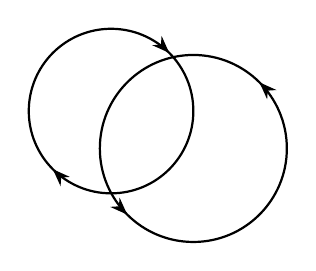
\begin{tikzpicture}[x=0.95cm, y=0.95cm, thick, baseline=(current bounding box.center)]
            \draw[postaction={decorate}, decoration={markings,
                mark=between positions 0.125 and 1 step 0.5 with {\arrow{Stealth[length=2.2mm]}}}]
                (1.80, -0.25) arc[start angle=0, end angle=360, radius=1.25];
            \draw[postaction={decorate}, decoration={markings,
                mark=between positions 0.375 and 1 step 0.5 with {\arrow{Stealth[length=2.2mm]}}}]
                (0.55, 0.25) arc[start angle=0, end angle=-360, radius=1.1];
        \end{tikzpicture}\hfill$\longrightarrow$\hfill
        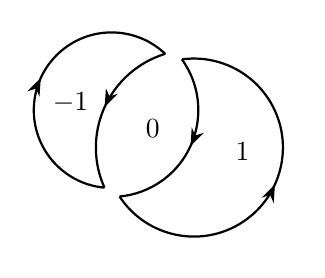
\begin{tikzpicture}[x=0.95cm, y=0.95cm, thick, baseline=(current bounding box.center)]
            % the part of the right circle outside the left one, then the part of the left circle inside the right one
            \draw[mid arrow] (-0.443, -0.905) arc[start angle=-146.6, end angle=97.7, radius=1.19];
            \draw[mid arrow] (0.390, 0.929) arc[start angle=35.8, end angle=-84.7, radius=1.16];
            % the part of the left circle outside the right one, then the part of the right circle inside the left one
            \draw[mid arrow] (-0.646, -0.786) arc[start angle=-95.3, end angle=-313.6, radius=1.04];
            \draw[mid arrow] (0.167, 1.003) arc[start angle=107.0, end angle=204.1, radius=1.31];
            \node at (1.2, -0.3) {$1$};
            \node at (0, 0) {$0$};
            \node at (-1.1, 0.35) {$-1$};
        \end{tikzpicture}\hfill\hfill
        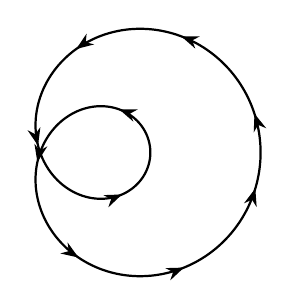
\begin{tikzpicture}[x=0.7cm, y=0.7cm, thick, baseline=(current bounding box.center)]
            \draw[loop arrows] plot[domain=0:360, samples=361, variable=\t]
                ({cos(\t) + 1.5*cos(2*\t)}, {sin(\t) + 1.5*sin(2*\t)});
        \end{tikzpicture}\hfill$\longrightarrow$\hfill
        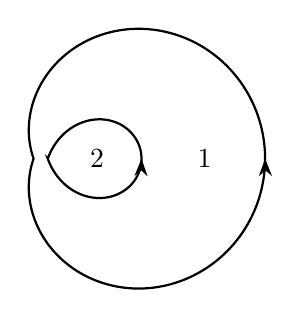
\begin{tikzpicture}[x=0.7cm, y=0.7cm, thick, baseline=(current bounding box.center)]
            % e^{it} + 1.5 e^{2it} crosses itself at t = arccos(-1/3); its two loops are pulled slightly apart
            \begin{scope}[shift={(0.5, 0)}, scale=1.05, shift={(-0.5, 0)}]
                \draw[mid arrow] plot[domain=-109.47:109.47, samples=181, variable=\t]
                    ({cos(\t) + 1.5*cos(2*\t)}, {sin(\t) + 1.5*sin(2*\t)}) -- cycle;
            \end{scope}
            \begin{scope}[shift={(-0.45, 0)}, scale=0.85, shift={(0.45, 0)}]
                \draw[mid arrow] plot[domain=109.47:250.53, samples=121, variable=\t]
                    ({cos(\t) + 1.5*cos(2*\t)}, {sin(\t) + 1.5*sin(2*\t)}) -- cycle;
            \end{scope}
            \node at (-0.45, 0) {$2$};
            \node at (1.5, 0) {$1$};
        \end{tikzpicture}
    \end{center}
    Do the same for the figures below.
    對下面的圖做同樣的事。
    
\answerpar\mbox{\Problem{\loopfigJ{loop dotted}{scale=1.3}}~\loopfigJ{loop arrows}{scale=0.85}}\hfill
% Ans (2 points): figure J in ../1030/loop-key.pdf; 3 crossings; 2 loops (ccw, cw); the bounded regions have winding numbers -1, 0, 0, 1.
\mbox{\Problem{\loopfigL{loop dotted}{scale=0.99}}~\loopfigL{loop arrows}{scale=0.85}}\hfill
% Ans (2 points): figure L in ../1030/loop-key.pdf; 4 crossings; 3 loops (ccw, ccw inside 1, cw); the bounded regions have winding numbers -1, 0, 1, 1, 2.
\mbox{\Problem{\loopfigO{loop dotted}{scale=1.04}}~\loopfigO{loop arrows}{scale=0.85}}\hfill
% Ans (2 points): figure O in ../1030/loop-key.pdf; 6 crossings; 4 loops (cw, cw inside 1, ccw, ccw); the bounded regions have winding numbers -2, -1, -1, -1, 0, 1, 1.
\mbox{\Problem{\loopfigS{loop dotted}{scale=0.76}}~\loopfigS{loop arrows from 3mm}{scale=0.85}}
% Ans (2 points): the hummingbird; 3 crossings (the curls on the wing); 4 loops, all counterclockwise: the outline and the 3 curls inside it;
% the bounded regions have winding numbers 1 (the body and a small pocket next to a curl) and 2 (inside each curl).
% Grading: one point for the loops (disjoint, keeping the direction of every arc)
% and one point for the winding numbers (every bounded region must carry the right one).

\problemlabel{$\strut$}
    Now the other way around.
    You are given the winding numbers of each region,
    and you need to mark the direction of each closed curve.

\answerpar\mbox{\Problem{\windfigT{loop dotted}{scale=1.3}{}}~\windfigT{thick}{}{\windnumsT}}\hfill
% Ans: the top circle counterclockwise, the lower left circle clockwise, the lower right circle counterclockwise.
\mbox{\Problem{\windfigQ{loop dotted}{scale=1.3}{}}~\windfigQ{thick}{}{\windnumsQ}}
% Ans: the left ellipse counterclockwise, the middle ellipse tilted up to the right clockwise,
% the middle ellipse tilted up to the left counterclockwise, the right ellipse counterclockwise.

\answerpar\mbox{\Problem{\windfigF{loop dotted}{scale=0.7}{}}~\windfigF{thick}{scale=0.7}{\windnumsF}}
% Ans: by the direction of each curve's center from the origin: 319 ccw, 31 cw, 103 cw, 175 ccw, 247 cw
% (the curves are drawn in this order in \windfigF, rotated by 0, 72, 144, 216, 288 degrees).

\problemlabel{$\strut$}
    TaTung computes Schwarzian derivatives:
    for $f$ with $f' \ne 0$, $S(f) = (f''/f')' - (f''/f')^2/2$.
    TaTung 計算 Schwarzian derivative：對 $f' \ne 0$ 的 $f$，$S(f) = (f''/f')' - (f''/f')^2/2$。
\problem{8}
    $S(f)$ for $f(z) = e^{(q_2+1)z}$.
    求 $f(z) = e^{(q_2+1)z}$ 的 $S(f)$。
% Ans: -(q_2 + 1)^2/2 (f''/f' is the constant q_2 + 1).
\problem{12}
    $S(f)$ for $f(z) = z^{q_7+2}$, $z \ne 0$.
    求 $f(z) = z^{q_7+2}$（$z \ne 0$）的 $S(f)$。
% Ans: with m = q_7 + 2, f''/f' = (m - 1)/z, so S(f) = -(m - 1)/z^2 - (m - 1)^2/2z^2 = (1 - m^2)/2z^2.
\problem{5}
    $S(f)$ for $f(z) = (2z + 1)/(z + 3)$.
    求 $f(z) = (2z + 1)/(z + 3)$ 的 $S(f)$。
% Ans: 0 (f''/f' = -2/(z + 3); every Mobius transformation has Schwarzian 0).
\problem{5}
    $S(f)$ for $f(z) = \tan z$.
    求 $f(z) = \tan z$ 的 $S(f)$。
% Ans: 2 (f''/f' = 2 tan z, so S = 2 sec^2 z - 2 tan^2 z = 2).

\problemlabel{$\strut$}
    DongHwa continues a function analytically by re-expanding power series.
    Let $h$ be holomorphic on $\CC \setminus \ZZ$,
    and let $h(z) = \sum_{n\ge0}a_n(z - i)^n$ be its Taylor series about $i$;
    by Taylor's theorem it converges on the largest open disk centered at $i$ that contains no integer.
    Each jump below moves the center to a point inside the current disk of convergence and re-expands $h$ there.
    DongHwa 用重新展開冪級數的方法做 analytic continuation。
    設 $h$ 在 $\CC \setminus \ZZ$ 上 holomorphic，$h(z) = \sum_{n\ge0}a_n(z - i)^n$ 是它在 $i$ 的 Taylor series；
    由 Taylor's theorem，它在以 $i$ 為圓心、不含任何整數的最大開圓盤上收斂。
    下面每一次「跳」都是把圓心移到目前收斂圓盤內的一點，再把 $h$ 在那裡重新展開。
\problem{3}
    Can DongHwa get from $i$ to $1000 + i$ in at most $1010$ jumps? Answer Y or N.
    DongHwa 能不能在 $1010$ 次以內從 $i$ 跳到 $1000 + i$？回答 Y 或 N。
% Ans: Y. Along the line Im z = 1 every disk has radius at least 1, so 1010 equal jumps of length 1000/1010 < 1 suffice
% (1001 jumps would also do).

\problemlabel{$\strut$}
    FengChia studies where the roots of $p'$ can be.
    Let $p(z) = c(z - z_1)(z - z_2)\cdots(z - z_n)$ with $c \ne 0$ and $n \ge 2$.
    FengChia 研究 $p'$ 的根可能在哪裡。
    設 $p(z) = c(z - z_1)(z - z_2)\cdots(z - z_n)$，其中 $c \ne 0$、$n \ge 2$。
\problem{10}
    Write $p'(z)/p(z)$ as a sum over the roots $z_k$.
    把 $p'(z)/p(z)$ 寫成對所有根 $z_k$ 的和。
% Ans: sum_{k=1}^n 1/(z - z_k).
\problem{15}
    Let $w$ be a root of $p'$ that is not a root of $p$.
    Take the complex conjugate of $p'(w)/p(w) = 0$, and find positive numbers $t_k$ with $\sum_k t_k(w - z_k) = 0$.
    設 $w$ 是 $p'$ 的根但不是 $p$ 的根。
    對 $p'(w)/p(w) = 0$ 取共軛，找出正數 $t_k$ 使得 $\sum_k t_k(w - z_k) = 0$。
% Ans: t_k = 1/|w - z_k|^2, since the conjugate of 1/(w - z_k) is (w - z_k)/|w - z_k|^2.
\problem{15}
    Write $w$ as a weighted average of the $z_k$, with nonnegative weights adding up to $1$.
    把 $w$ 寫成 $z_k$ 的加權平均，權重非負且和為 $1$。
% Ans: w = sum_k t_k z_k / sum_j t_j. So every root of p' lies in the convex hull of the roots of p (the Gauss--Lucas theorem);
% roots of p' that are also roots of p lie there trivially.

\problemlabel{$\strut$}
    TaiPei uses Hadamard's three-circle theorem:
    if $f$ is holomorphic on the closed annulus $r_1 \le |z| \le r_3$
    and $M(r)$ denotes the maximum of $|f|$ on the circle $|z| = r$, then for $r_1 \le r_2 \le r_3$,
    \[
        \log M(r_2) \le \frac{\log(r_3/r_2)\log M(r_1) + \log(r_2/r_1)\log M(r_3)}{\log(r_3/r_1)}.
    \]
    In each problem, $f$ is holomorphic on the closed annulus between the two given circles.
    TaiPei 使用 Hadamard's three-circle theorem：
    若 $f$ 在閉環形區域 $r_1 \le |z| \le r_3$ 上 holomorphic，$M(r)$ 是 $|f|$ 在圓 $|z| = r$ 上的最大值，
    則對 $r_1 \le r_2 \le r_3$ 上式成立。
    每一題中的 $f$ 都在兩個給定的圓之間的閉環形區域上 holomorphic。
\problem{10}
    Suppose $|f| \le 1$ on $|z| = 1$ and $|f| \le 4^{q_8+1}$ on $|z| = 4$.
    What upper bound for $|f|$ on $|z| = 2$ does the theorem give?
    設在 $|z| = 1$ 上 $|f| \le 1$，在 $|z| = 4$ 上 $|f| \le 4^{q_8+1}$。
    這個定理給出 $|f|$ 在 $|z| = 2$ 上的什麼上界？
% Ans: 2^{q_8+1}: log M(2) <= (log 2 * 0 + log 2 * (q_8 + 1) log 4)/log 4 = (q_8 + 1) log 2;
% since 2 is the geometric mean of 1 and 4, the bound is the geometric mean of 1 and 4^{q_8+1}.
\problem{10}
    Suppose $|f| \le 8$ on $|z| = 1$ and $|f| \le 1$ on $|z| = 8$.
    What upper bound for $|f|$ on $|z| = 2$ does the theorem give?
    設在 $|z| = 1$ 上 $|f| \le 8$，在 $|z| = 8$ 上 $|f| \le 1$。
    這個定理給出 $|f|$ 在 $|z| = 2$ 上的什麼上界？
% Ans: 4: log M(2) <= (log 4 * log 8 + log 2 * 0)/log 8 = log 4.
\problem{3}
    For $f(z) = z^n$ with an integer $n$, does equality hold in the theorem for all $r_1 \le r_2 \le r_3$? Answer Y or N.
    對 $f(z) = z^n$（$n$ 為整數），定理中的不等式是否對所有 $r_1 \le r_2 \le r_3$ 都取等號？回答 Y 或 N。
% Ans: Y (log M(r) = n log r is linear in log r).

\problemlabel{$\strut$}
    ShihChien computes $\sum_{n\ge1}n^{-2}$.
    Let $g(z) = \pi\cot(\pi z)z^{-2}$, and for $N = 1, 2, \ldots$
    let $C_N$ be the boundary of the square with vertices $(N + 1/2)(\pm1 \pm i)$, traversed counterclockwise.
    You may use that $|\cot(\pi z)| \le 2$ on every $C_N$.
    ShihChien 要計算 $\sum_{n\ge1}n^{-2}$。
    令 $g(z) = \pi\cot(\pi z)z^{-2}$；對 $N = 1, 2, \ldots$，
    令 $C_N$ 是頂點為 $(N + 1/2)(\pm1 \pm i)$ 的正方形的邊界，逆時針方向。
    可以直接使用：在每個 $C_N$ 上 $|\cot(\pi z)| \le 2$。
\problem{10}
    Find the coefficient of $z^{-1}$ in the Laurent series of $g$ about $0$.
    求 $g$ 在 $0$ 的 Laurent series 中 $z^{-1}$ 的係數。
% Ans: -pi^2/3 (pi cot(pi z) = 1/z - pi^2 z/3 - ...).
\problem{8}
    For an integer $n \ne 0$, find the coefficient of $(z - n)^{-1}$ in the Laurent series of $g$ about $n$.
    對整數 $n \ne 0$，求 $g$ 在 $n$ 的 Laurent series 中 $(z - n)^{-1}$ 的係數。
% Ans: 1/n^2 (pi cot(pi z) = 1/(z - n) + ... near n).
\problem{12}
    What upper bound for $\bigl|\oint_{C_N}g(z)\,dz\bigr|$ does the ML-inequality give?
    ML-inequality 給出 $\bigl|\oint_{C_N}g(z)\,dz\bigr|$ 的什麼上界？
% Ans: |z| >= N + 1/2 on C_N, so |g| <= 2 pi/(N + 1/2)^2; L = 8(N + 1/2); the bound is 16 pi/(N + 1/2), which tends to 0.
\problem{8}
    The integral $\oint_{C_N}g(z)\,dz$ is $2\pi i$ times the sum, over all poles of $g$ inside $C_N$,
    of the coefficients found in the previous two problems.
    Let $N \to \infty$ to find $\sum_{n\ge1}n^{-2}$.
    積分 $\oint_{C_N}g(z)\,dz$ 等於 $2\pi i$ 乘以前兩題的係數對 $C_N$ 內所有 poles 的和。
    令 $N \to \infty$，求 $\sum_{n\ge1}n^{-2}$。
% Ans: pi^2/6, since oint_{C_N} g dz = 2 pi i (-pi^2/3 + 2 sum_{n=1}^N 1/n^2) -> 0.

\clearpage

\baselineskip3em
\lineskip2em
\raggedright
Engineering Mathematics: Complex Variable, second mock midterm answer sheet
工程數學：複變期中考第二次模擬考答案卷
\answersheet\par

\end{document}
